\section{Metric Graphs}
\label{ch1:sec1}

This chapter is dedicated to the introduction of the basic principles about metric graphs and resulting concepts, which we need for a reasonable derivation of numerical methods on these structures. The following material has been adopted from \cite[chapter~1]{BerkolaikoKuchment:2013} unless otherwise noted. \\

We define a graph $\Gamma$ as an ordered pair $(\mathcal{V}, \mathcal{E})$, where $\mathcal{V} = \{v_i\}$ is a finite set of points, which we call vertices, and $\mathcal{E} = \{e_j\}$ is a set of segments connecting some of the vertices, which we call edges. In the following we will use the notation $E \coloneqq \left\lvert \mathcal{E} \right\rvert$ for the number of edges and $V \coloneqq \left\lvert \mathcal{V} \right\rvert$ for the number of vertices. \\
Each edge $e \in \mathcal{E}$ can be identified with a pair $(v, w)$ of vertices $v, w \in \mathcal{V}$, which it connects. A graph $\Gamma = (\mathcal{V}, \mathcal{E})$ is called directed graph, if each of its edges $e \in \mathcal{E}$ is assigned a direction, which means that each edge can only be followed in one direction. In this case, the order of the pair of vertices $(v, w)$ describing an directed edge $e$ is important, so that the set of directed edges $\mathcal{E}$ can be uniquely described as a set of ordered pairs $\mathcal{E} = \{e_i\}_{i = 1, \ldots, E} = \{(v^{o}_{i}, v^{t}_{i})\}_{i = 1, \ldots, E}$, where the first vertex $v^{o}_{i}$ is called the origin vertex and the second vertex $v^{t}_{i}$ is called the terminal vertex of the corresponding edge $e_i$. These origin and terminal vertex of a directed edge can be specified via functions $o \colon \mathcal{E} \to \mathcal{V}$ and $t \colon \mathcal{E} \to \mathcal{V}$, i.e. a directed edge $e = (v^{o}, v^{t})$ begins at $o(e) = v^{o}$ and ends at $t(e) = v^{t}$. We define the set of incoming directed edges at a vertex $v$ as the set of directed edges satisfying $t(e) = v$, if $o(e) = v$, the directed edge $e$ is called outgoing at the vertex $v$. \\
A graph $\Gamma = (\mathcal{V}, \mathcal{E})$ is non-directed if each of its edges $e \in \mathcal{E}$ can be followed in both directions. In this case, the order of the two connected vertices describing an edge is unimportant, i.e. $e = (v, w) = (w, v)$ with $v, w \in \mathcal{V}$. \\
In general, graphs are represented as one-dimensional drawings of points and lines, where the points represent the vertices and the lines represent the edges. \cref{fig1:f1} shows an undirected graph. In a directed graph, an arrow at the end of an edge indicates which direction is assigned to the corresponding edge, as shown in \cref{fig1:f2}. 

\begin{figure}[H]
    \begin{subfigure}[b]{0.4\textwidth}
        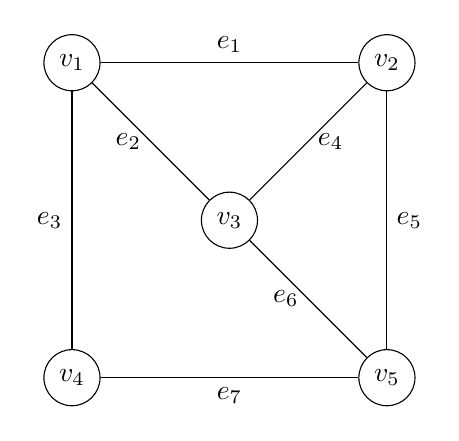
\begin{tikzpicture}
            % vertices
            \node[shape=circle,draw=black] (v1) at (0,4) {$v_1$};
            \node[shape=circle,draw=black] (v2) at (4,4) {$v_2$};
            \node[shape=circle,draw=black] (v3) at (2,2) {$v_3$};
            \node[shape=circle,draw=black] (v4) at (0,0) {$v_4$};
            \node[shape=circle,draw=black] (v5) at (4,0) {$v_5$};
            
            % edges
            \path [-](v1) edge node[above] {$e_1$} (v2);
            \path [-](v1) edge node[left] {$e_2$} (v3);
            \path [-](v1) edge node[left] {$e_3$} (v4);
            \path [-](v2) edge node[right] {$e_4$} (v3);
            \path [-](v2) edge node[right] {$e_5$} (v5);
            \path [-](v3) edge node[left] {$e_6$} (v5);
            \path [-](v4) edge node[below] {$e_7$} (v5);
        \end{tikzpicture}
        \caption{Non-directed graph}
        \label{fig1:f1}
    \end{subfigure}
    \hfill
    \begin{subfigure}[b]{0.4\textwidth}
        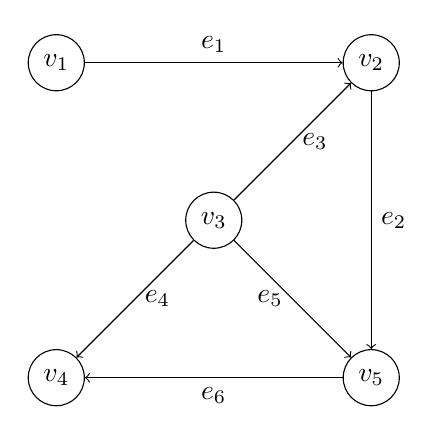
\begin{tikzpicture}
            % vertices
            \node[shape=circle,draw=black] (v1) at (0,4) {$v_1$};
            \node[shape=circle,draw=black] (v2) at (4,4) {$v_2$};
            \node[shape=circle,draw=black] (v3) at (2,2) {$v_3$};
            \node[shape=circle,draw=black] (v4) at (0,0) {$v_4$};
            \node[shape=circle,draw=black] (v5) at (4,0) {$v_5$};
            
            % edges
            \path [->](v1) edge node[above] {$e_1$} (v2);
            \path [->](v2) edge node[right] {$e_2$} (v5);
            \path [->](v3) edge node[right] {$e_3$} (v2);
            \path [->](v3) edge node[right] {$e_4$} (v4);
            \path [->](v3) edge node[left] {$e_5$} (v5);
            \path [->](v5) edge node[below] {$e_6$} (v4);
        \end{tikzpicture}
        \caption{Directed graph}
        \label{fig1:f2}
    \end{subfigure}
    \caption{Two different types of graphs.}
\end{figure}

It is necessary for some considerations that a non-directed graph will be considered as a directed graph by assigning two directed edges $e$ and $\overline{e}$ with opposite directions to each edge of the non-directed graph $\Gamma$, as shown in \cref{fig2}. We denote the resulting directed graph by $\widetilde{\Gamma}$.

\begin{figure}[H]
    \begin{subfigure}[b]{0.4\textwidth}
        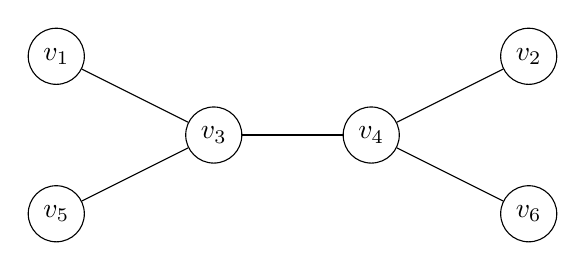
\begin{tikzpicture}
            % vertices
            \node[shape=circle,draw=black] (v1) at (-3,1) {$v_1$};
            \node[shape=circle,draw=black] (v2) at (3,1) {$v_2$};
            \node[shape=circle,draw=black] (v3) at (-1,0) {$v_3$};
            \node[shape=circle,draw=black] (v4) at (1,0) {$v_4$};
            \node[shape=circle,draw=black] (v5) at (-3,-1) {$v_5$};
            \node[shape=circle,draw=black] (v6) at (3,-1) {$v_6$};
            
            % edges
            \path [-](v1) edge (v3);
            \path [-](v5) edge (v3);
            \path [-](v3) edge (v4);
            \path [-](v2) edge (v4);
            \path [-](v6) edge (v4);
        \end{tikzpicture}
        \caption{Non-directed graph }
    \end{subfigure}
    \hfill
    \begin{subfigure}[b]{0.4\textwidth}
        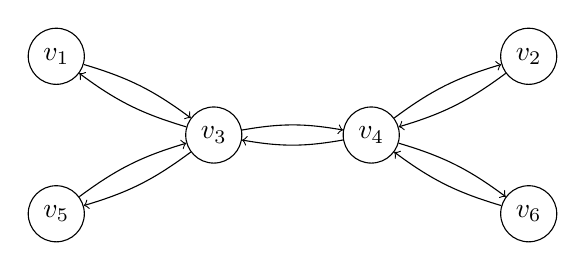
\begin{tikzpicture}
            % vertices
            \node[shape=circle,draw=black] (v1) at (-3,1) {$v_1$};
            \node[shape=circle,draw=black] (v2) at (3,1) {$v_2$};
            \node[shape=circle,draw=black] (v3) at (-1,0) {$v_3$};
            \node[shape=circle,draw=black] (v4) at (1,0) {$v_4$};
            \node[shape=circle,draw=black] (v5) at (-3,-1) {$v_5$};
            \node[shape=circle,draw=black] (v6) at (3,-1) {$v_6$};
            
            % edges
            \path [->](v1) edge [bend left = 10] (v3);
            \path [->](v3) edge [bend left = 10] (v1);
            \path [->](v5) edge [bend left = 10] (v3);
            \path [->](v3) edge [bend left = 10] (v5);
            \path [->](v3) edge [bend left = 10] (v4);
            \path [->](v4) edge [bend left = 10] (v3);
            \path [->](v2) edge [bend left = 10] (v4);
            \path [->](v4) edge [bend left = 10] (v2);
            \path [->](v6) edge [bend left = 10] (v4);
            \path [->](v4) edge [bend left = 10] (v6);
        \end{tikzpicture}
        \caption{Directed graph}
    \end{subfigure}
    \caption{Two different types of graphs.}
    \label{fig2}
\end{figure}

The graph  satisfies the condition that at each vertex  v the numbers of incoming and outgoing directed edges are equal: (the notation dv := dv/2 will be used in this situation). The set of directed edges of  is symmetric in the sense that  if and only if there is another directed edge such that o(b) = t(b) and t(b) = o(b). The directed edge b is called the reversal of b. The operation of reversal is reflexive: b = b.
\\
A vertex $w \in \mathcal{V}$ is adjacent to a vertex $v \in \mathcal{V}$, denoted by $v \sim w$, if a suitable edge $e \in \mathcal{E}$ exists, so that $w$ can be reached from $v$ via this edge $e$. In the following we assume that a graph has no loops, which are edges that connect a vertex $v \in \mathcal{V}$ to itself, i.e. $v \sim v$, and no multi-edges, which are several equal edges between two vertices, i.e. $e_1, e_2 \in \mathcal{E}$ and $e_1 = e_2$. A graph $\Gamma = (\mathcal{V}, \mathcal{E})$ with $\mathcal{V} = \{v_i\}_{i = 1, \ldots, V}$ is fully specified by its $V \times V$ adjacency matrix $A^{\Gamma}$. The elements of the adjacency matrix are given by
\begin{equation}
    \label{adjacency matrix}
    A^{\Gamma}_{i, j}= \begin{cases} 1 & \text { if } v_i \sim v_j \\ 0 & \text { otherwise. } \end{cases}
\end{equation}
One sees immediately that the adjacency matrix of an non-directed graph is symmetric, since a vertex $v \in \mathcal{V}$ is adjacent to another vertex $w \in \mathcal{V}$ exactly when the other way round is also true, i.e. $v \sim w \Leftrightarrow w \sim v$. \\
The degree $d_{v_i}$ of a vertex $v_i \in \mathcal{V}$ is the number of edges emanating from it, i.e. $d_{v_i} = \sum_{v_j \in \mathcal{V}} A_{i, j}$. All degrees are assumed to be finite. We will denote by $D^{\Gamma}$ the degree matrix of the graph, which is a diagonal $V \times V$ matrix with the entries
\begin{equation}
    \label{degree matrix}
    D^{\Gamma}_{i, j} = d_{v_i} \, \delta_{v_j, v_i}
\end{equation}
where $\delta_{v_j, v_i}$ is the Kronecker delta. \\

The number of incoming (respectively, outgoing) directed edges at a vertex v is called incoming (resp.outgoing) degree of v and denoted  (resp. dov). Clearly, dov + div = dv.

A vertex is incident to an edge, denoted by $v \in e$, if the vertex $v \in \mathcal{V}$ is one of the two vertices the edge $e \in \mathcal{E}$ connects. We define for an non-directed graph $\Gamma = (\mathcal{V}, \mathcal{E})$ with $\mathcal{V} = \{v_i\}_{i = 1, \ldots, V}$ and $\mathcal{E} = \{e_i\}_{i = 1, \ldots, E}$ the $V \times E$ incidence matrix $B^{\Gamma}$ by  
\begin{equation}
    \label{incidence matrix non-directed}
    B^{\Gamma}_{i, j}= \begin{cases} 1 & \text { if } v_i \in e_j \\ 0 & \text { otherwise } \end{cases}
\end{equation}
and for a directed graph $\Gamma = (\mathcal{V}, \mathcal{E})$ with $\mathcal{V} = \{v_i\}_{i = 1, \ldots, V}$ and $\mathcal{E} = \{e_i\}_{i = 1, \ldots, E}$ we define the $V \times E$ incidence matrix $B^{\Gamma}$ by 
\begin{equation}
    \label{incidence matrix directed}
    B^{\Gamma}_{i, j}= \begin{cases} 1 & \text { if } e_j = (v_i, \cdot) \\ -1 & \text { if } e_j = (\cdot, v_i) \\ 0 & \text { if } v_i \notin e_j. \end{cases}
\end{equation}

% We also denote by $\mathcal{E}_v$ the set of all edges incident to the vertex $v$ (i.e., containing $v$). It is assumed that the degree (valence) dv = |Ev| of any vertex v is finite and positive. We hence exclude vertices with no edges coming in or going out.

So far we have considered graphs as discrete combinatorial objects. From now on we consider graphs as 1-dimensional complexes and the edges will be treated as 1-dimensional segments. If one considers graphs as 1D complexes, which we will often do, there exists a natural projection that maps the points x

%Grafik

Roughly speaking, we now imagine the edges $\mathcal{E}$ of a graph $\Gamma = (\mathcal{V}, \mathcal{E})$ not as abstract relations between the vertices $\mathcal{V}$, but rather as physical “wires” connecting them. For that we add a structure that equips $\Gamma$ with a topology and metric. 

\begin{definition}\label{metric graph}
    A graph $\Gamma = (\mathcal{V}, \mathcal{E})$ is said to be a metric graph, if each of its edges $e \in \mathcal{E}$ is assigned a positive length $l_e > 0$.
\end{definition}

%Having the length assigned, an edge e will be identified with a finite or infinite segment [0, le] of the real line with the natural coordinate xe along it. In most cases we will drop the subscript in the coordinate and call it x, which should not lead to any confusion. This enables one to interpret the graph Γ as a topological space (simplicial complex) that is the union of all edges where the ends corresponding to the same vertex are identified

